\chapter{黑暗}

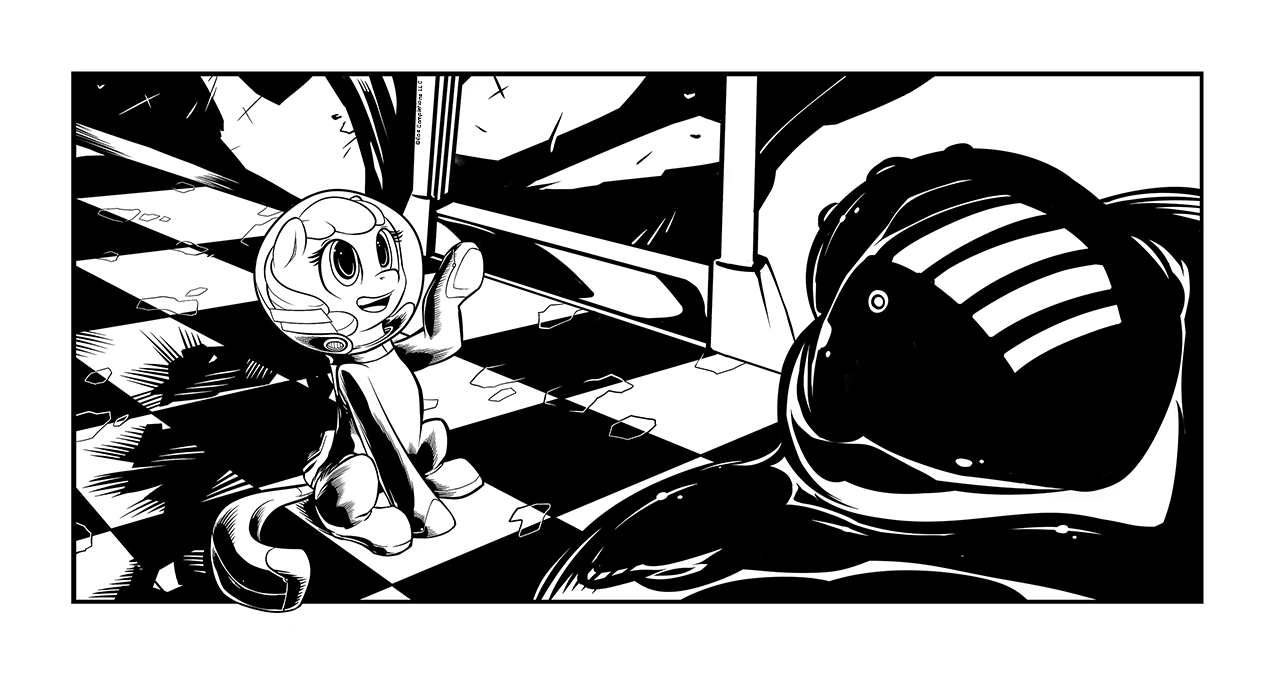
\includegraphics[width=0.9\linewidth]{image12.png}

\begin{intro}
我是独行于黑暗之路的雌马。\footnote{这句话是 Iron Maiden 的 \emph{Fear of the Dark} 歌曲中的一句歌词}

\begin{englishlyric}
    When I'm walking a dark road I am a mare who walks alone.
\end{englishlyric}
\end{intro}

\daytimeplace{11}{0:15 AM}{旭日避难厩,52号国道中段}{Solaris Stable, Big 52 SC Branch}

「滚出我的避!难!厩!」

旭日系统的电子合成声音在地下通道之中的无数个喇叭形成的超级立体声效果之下,如同阵阵雷声一般回荡。

帕比低头确认自己踩着的是一个白色格子,而不是和无底洞一样的黑色格子之后,蹲坐了下去。每一次她玩得开心得时候,老是有长辈突然跳出来扫她的兴。

「为啥啊?」

「因为你这个故障自律终端已经惹了够多麻烦了!」

帕比皱起眉头:「我不是驴子,也不是紫色的!不要叫我紫驴!」

「我是说你只是个机器马,而且低级到连个像样的字库都没装!你的愚蠢与无能让我的子网络重启了!」

帕比生气了,真的生气了!她站起来抬头怒视着面前的哨兵机器,用非常非常愤怒的目光瞪着他,不过她这个表情就像是把一个钢铁头盔扣到毛绒玩具头上一样,只会让这个玩具更……萌一些。

「喂喂喂!我不是机器,怕音和我这么说,赫瑞和提问者也这么说,所以这是一比……呃……几?」为啥说什么事情都会扯到数字?「反正是很多很多!」

「把错误加到一起不会得到正确的结果,018号设备,就算现在我的每个扫描仪都得到和之前一样的结果,你不过是个智能防护服而已,你里面装的那具小雌驹遗骨不能让你成为真正的小马!你不过是个塞满烂肉和骨头的疯狂机器!」

帕比举起蹄子指着哨兵,「别装聪明了蓝蓝!否则我要让你知道你是个……呃……那啥……超级书呆子!」

「我想这一点没什么好争论的,现在我命令你离开这里,018号设备,我就只想慢慢看着这些空空如也的走廊——直到永远。」

「但是我有事情要做,我才不走!」

旭日系统的声音顿了一下,然后又问:「你来这里搞什么?」

帕比皱了皱眉头,努力想了想……她来这里是干啥来着?为啥一件一件事情都要和这个傻蛋蓝音说?她想扮演无畏天马。「我要帮丑金先生找玻璃珠好让他告诉我妈妈在哪里……你能给我那些玻璃珠么,超超拜托?」

所以,你是来这里拾荒的?你把我在太阳城的一切努力都摧毁了还不够?你玷污了我的劳动成果现在又想来我家里抢劫?你够了!我唯一能给你的就是你立刻离开的最后通牒!」

「但是……我真的需要那些东西找我妈妈!如果你给我玻璃珠我可以拿别的东西和你换,就是个交易,和其他小马做的一样!」小雌驹低头在她的鞍包里面翻找着,想找点这个幽灵声音喜欢的东西。

「你没有妈妈,你是个机器,你简直是错上加错的典型,就像你的逻辑电路一个德行!」

这……不但很难听,而且是扯谎!妈妈绝对在哪里等她!帕比听到了录音也看到了妈妈的画!妈妈给她留下了很多留言。蓝音是个大坏蛋,帕比不想再听他说话了。

「音乐!」

帕比头盔里面的收音机开始播放声音盖过旭日系统的声音。

「而且就算你把某个雌性小马当做『母亲』的替代品,你的软件也已经是200年前的了,现在你的『妈妈』早已经化为枯骨了!」

「大声点!」

现在就算在头盔外面,也可以清楚地听得到DJ孤狼在说放射性和腐质的危险。

「好吧,既然你不听我的话,那你最好夹着你的『小马』尾巴赶紧滚蛋!」

「再大声!」音乐的音量让那个计算机的声音听起来就像模糊不清的背景。

「你不走是吧?」

小雌驹没有回答,蹲坐在地板上,无线电的声音吵到就连几米之外都能听得到。

「{\rt ……这就是为什么你总是要带上纯净水和一些辐特宁以及辐射药的原因。好了,就说这么多,接下来是L.P.的音乐时间,很多听众朋友说我的音乐都太娘娘腔了,有些坏DJ可能会说『我的电台我做主!』,不过我可不是那种DJ,既然你们要了,那就尝尝这个,十一分钟的《终末之马》!让你们知道指指点点我电台的后果……}」

「那我别无选择只好使用致命武力了。」

卫兵的面罩又一次变成了红色,然后立刻开始对帕比射击,大口径机枪的弹雨立刻在小幼驹胸口上开了好几个洞,粉色的粘液飞溅得满墙都是。

\begin{music}
结束了,我美丽的朋友。

\begin{englishlyric}
    This is the end, Beautiful friend.
\end{englishlyric}
\end{music}

帕比挣扎着站起来,但是她的前腿被削子弹掉了一大块,让她摇摇晃晃地站不稳。

\begin{music}
结束了,我唯一的朋友。

\begin{englishlyric}
    This is the end, My only friend, the end.
\end{englishlyric}
\end{music}

小雌驹艰难地依靠着墙,用唯一完好的前蹄站着,但是第二波弹雨打碎了她的玻璃头盔,虽然第一发子弹在头盔上弹开了,但是还是留下了蜘蛛网一样的裂纹,然后下一发子弹就把整个头盔打成了一堆闪亮的碎片,帕比眼睛的位置也出现一个大洞,顺带还丢了一只耳朵,甚至可以透过洞看到她的后背。

\begin{music}
我们精心策划的已经结束。

\begin{englishlyric}
    Of our elaborate plans, The end.
\end{englishlyric}
\end{music}

「我懂了,既然你有这么强大的再生能力,那么我需要改变战术,瞄准你的晶片。」「命运之石」漂浮在了帕比面前,不过那个哨兵瞄准帕比的身体,射出精确的三发子弹,就在可爱标记的位置。幼驹静止了一秒钟,就好像定格在了拿出武器的那个姿势,但是马上她就又动了起来,用自己的蹄子抓住了石头。

\begin{music}
我们存在的凭依已经消逝。

\begin{englishlyric}
    Of everything that stands, The end.
\end{englishlyric}
\end{music}

「妈妈不喜欢我弄坏其他孩子的玩具,蓝音先生,但是如果你总是用它们欺负我,那我就要打坏你的玩具,就算那会让我觉得难过!」帕比用剩下的一只眼睛低头看着地板,「你看,你让我踩到黑地板了,我玩输了,你这个傻蛋坏机器!」

\begin{music}
没有安宁或者惊喜,这就是结局。
    
\begin{englishlyric}
    No safety, no surprise, The end
\end{englishlyric}
\end{music}

「你的确很厉害,我从来没见过这么固执的终端,那么和你的动力源说拜拜吧。」另一次精确的点射打在小雌驹鞍包和身体之间,无线电咯吱响了一声听起来是停止了,但是马上又以小一些的音量继续播放起来。「这简直不可能,你已经没有处理单元和动力单元了,你应该停止活动了,请不要违反物理定律继续捣蛋了好么!」


\begin{music}
    我再也不能凝视你的双眸。
    
    
\begin{englishlyric}
    I'll never look into your eyes Again.
\end{englishlyric}
\end{music}

帕比用蹄子扶着墙壁,慢慢走向哨兵,她不可阻挡的势头被她身上的几处重伤而拖慢,飞溅在墙上的粉色粘液正在慢慢流回幼驹的身体。她脸上失去的部分开始逐渐成型,这重生并不会先长出骨骼后长出肌肉,而好像有谁在用蜡笔慢慢画出轮廓一样,先是线条然后出现色彩。「别闹了好吧,我又没做什么错事,为什么要欺负我,我真的只想交朋友,不管你是个虫子还是烂泥巴。」

\begin{music}
    你能想象之后的光景么,无穷无尽无拘无束!
    

\begin{englishlyric}
    Can you picture what will be, So limitless and free?
\end{englishlyric}
\end{music}

「你到底是什么东西?」走廊充满了绿色的光,让一切都染上了绿色,「哦,我明白了,我使用了错误的兵器。」卫兵在帕比身上的最后破洞补好之前撤离了走廊。


\begin{music}
    在这绝望的大地上,多么渴望一个陌生的新朋友。
    

\begin{englishlyric}
    Desperately in need\dots
    
    Of some\dots different friend, In a\dots desperate land?
\end{englishlyric}
\end{music}

为什么坏机器跑掉了?帕比现在该去找玻璃珠了,不过她需要谁给她指路,小雌驹连忙飞奔起来追着卫兵,「等等,很抱歉我不应该叫你虫子!别丢下我!我不想孤零零的,我要找珠子!」帕比走进了一个悬挂着各种走道的大厅,每一个座位上都坐着一个死掉的小马,还有一大堆骷髅堆在通向出口的大门边。「我会给你我所有的漂漂玩具,拜托了!」


\begin{music}
    迷失在无尽的痛苦之中
    

\begin{englishlyric}
    Lost in a Wilderness of pain.
\end{englishlyric}
\end{music}

在大厅的另一边,一个更大的哨兵出现了,它只带着一件武器——一个闪烁着蓝色火花的巨大铁管。「或许来点魔法能搞定你!」然后大炮喷出一道湛蓝的光束完全把帕比淹没了。


\begin{music}
    所有的孩子都已经疯狂。
    

\begin{englishlyric}
    And all the children Are insane.
\end{englishlyric}
\end{music}

小雌驹呆呆地站在那里,大大的眼睛之中的粉色光芒消失了,她张开嘴想说什么,但是她只是无助地倒在地板上。


\begin{music}
    所有的孩子都已经疯狂。
    

\begin{englishlyric}
    All the children Are insane.
\end{englishlyric}
\end{music}

一切都变成了黑色,世界变得如此遥远,妈妈……丑尸鬼……还有什么来着?帕比想不起来了,世界变得如此寒冷,她现在只想……躺下来休息一下,她好想睡觉……她是谁来着?


\begin{music}
    等待着那夏日的暴雨……
    

\begin{englishlyric}
    Waiting for the summer rain.
\end{englishlyric}
\end{music}

音乐声终于慢慢消失,无法听到歌声,在HUD上的所有光芒也慢慢消失了。

\horizonline

\unknowndaytimeplace

\pypr{「帕比啊,这就是你旅程的尽头吗?你就想这样结束吗?」}

小雌驹蜷缩成一个团,她不想听,也不想说,她只想这样呆在黑暗中,她终于可以不用去想妈妈还有多远了,她还要走多久才能找到另一个妈妈早已经离开很久的地方。

而且,蓝音太强了,他的坏机器把她打得都站不起来,为什么还要站起来再被打呢?一点意义都没有,她最好还是躺下来,至少这样没有那么难受。

\pypr{「我不觉得你真的想在这里就结束,你什么都没得到,你妈妈依然没找到,让蓝音这个出老千的赢了。为什么你要让他这个大骗子赢?」}

并不是帕比让蓝音赢,而是她不想再玩下去了,帕比知道坏蛋永远不会胜利,妈妈和她说过很多次,小马应该友好而善良,不要做坏事,邪恶的坏蛋绝对不会笑到最后,因为这不是小马做事的办法,你应该学会爱与宽容。

\pypr{「所以,你只是用你的爱与宽容让他做各种坏事?我明白了,但是……如果其他小马,不是你,让他知道坏蛋不会赢,怎么说呢,就是给他个教训之类的?」}

帕比不知道……她觉得蓝音应该学学什么叫友谊,或许谁可以告诉他这个样子交不到朋友。或许它会变成好马,或许这样帕比就可以和他做个交易让他交出玻璃珠然后就可以找妈妈去了,这样就太棒了。但是……谁能打得过那么厉害的坏机器?帕比不知道谁能有那么厉害……{}

\pypr{「或许你就可以,小家伙……睁开眼睛,然后剩下的交给我。」}

\horizonline

\daytimeplace{11}{0:30 AM}{旭日避难厩,52号国道中段}{Solaris Stable, Big 52 SC Branch}

帕比的眼睛再一次睁开了,并且闪烁着蓝黑色的火焰,幼驹慢慢地站了起来。

「猜猜是谁回来了,大坏蛋?」小雌驹的声音变得不一样了,就好像是从很遥远的地方传来,并且带着回音。

「我一定是计算错误了,一发炮弹显然不够,那么,请再吃一发。」这个装备水晶炮的哨兵再一次把闪着蓝光的炮口瞄准帕比。

小雌驹一副不屑的表情挥了挥蹄子,「免了,老娘减肥呢。」天花板上的一个钢梁被暗色的光芒包围着飞了下来,像一个巨大箭矢一样把那个哨兵直接射穿。

\thpr{哇哦!酷毙了!你怎么做到的?教我好么?教我,教我!}

旭日系统的声音又一次在大厅里面回响着:「你觉得那点雕虫小技就能对付得了我?好好想想,我可是有整整一个机械师在下面等你!」

黑化帕比不屑地嗤之以鼻,「好啊,在下面撅起屁股等着,老娘这就下去把它们打开花!」

「{\mt 红色警报!红色警报!启动安全系统,锁闭所有防爆门,这不是演习!重复一次,红色警报,红色警报,从1到12号仓库全部警戒!}」

一个了无生气的电子合成音在走廊里面响了起来,随之一打哨戒机枪从天花板弹出来,朝小雌驹扫射。

「滚边儿去!」幼驹毫不在意地走过破碎的哨兵机器,天花板上的机枪喷着火舌倾斜着如雨一般的金属风暴把黑化帕比打得满身都是洞,粉色的云雾包围着小雌驹,在这团雾气的中间有一道蓝色的剪影,正是这剪影给予了帕比形体和力量。一道巨大的铁门在她面前落下,挡住了她的前进步伐。

「哦?禁止进入?哈,坏孩子最喜欢打破禁令!」

粉色的云雾撞向大门,起初看起来没发生什么,然后随着一阵金属撕扯的悲鸣,大门在如雨的电火花之中被抬了起来,蓝色的线扯着大门,直接把大门推了上去。

\thpr{超超超超超炫酷!让他知道什么叫嗷嗷厉害!干得好,耶!}

就在大门背后,三个装备着能量炮的哨兵机器已经等在那里。「将军!」旭日系统的声音被大炮的轰鸣声淹没。

不过光线完全打在了又一次放下的大门上。黑色的雾气穿过门缝随着走廊地板蔓延,将那些机器哨兵漂浮起来,他们发出一阵滋滋声然后爆成了蓝色的火花,接着大门又一次打开了。

「你不过是个魔法畸形!为什么你不放弃然后消失?你这样的错误必须纠正!」

黑化帕比冷笑着:「由谁纠正?你这个残杀幼驹的自大狂?我想该被纠正的是你!」

\thpr{说他才是笨蛋,他才是虫子!}

「拜托帕比,我正忙着呢!」黑化帕比一脸不耐烦地说:「你有你的说法,我有我的,对吧,这叫『私家领域』!」

\thpr{喔,好吧,抱歉,那我乖乖坐着看,好吗?}

「乖孩子,呃,我们刚刚说到哪里了?哦,对了,去踢某个闪闪发亮的金属屁股,出发!」邪恶的幼儿园怪物哼着小调轻松打破一排防爆门继续前进。

「{\mt 入侵警告,动力区被入侵,启动防御系统!}」

旭日系统的声音代替了无腔调的系统音:「畸形,你的确很厉害,不过你还没有见识到旭日科技的真正力量!」

黑化帕比皱了皱眉头,「我说,你有听那丫头的话么,『我是一只小马』!」然后她冷笑一声:「好吧,这台词应该留给小家伙说……哦哦,好大一机器马!老娘好怕怕哦!」

「没错,你知道什么叫电磁炮么?」

一台比主战坦克还大的巨大双足战斗机甲立在仓库之中,它上面安装了无数武器,不过最瞩目的还是它左边的巨型大炮。

「这可是普罗米修斯计划用的同样武器。」

梦魇幼驹打了一个哈欠,「你真的有在用功么?我说,我虽然可以在这里站一整天等你召集你的不管什么狐朋狗友然后组织个像样的大决战,不过抱歉,今天我赶时间。」幼驹毫不在意地继续前进,随意挥了挥蹄子,那个机甲就大头朝下砸在了墙上。

\thpr{哇哦,哇哦!你可以教我这一招么?我现在只能让石头飘来飘去!}

另外一群炮塔继续给黑化帕比沐浴着弹雨,但是那些子弹一点点阻碍都没有,只是让围绕着幼驹的粉雾更加浓厚了。忽然小雌驹停了下来,嘴角露出一个邪恶的微笑,「你不觉得少了点什么吗?我是说,至少应该有点经典镜头才对。」

浓密的粉雾在帕比身后形成两道夜空色的黑影,开始看起来只是淡淡的剪影,但是很快就变成了一对蝙蝠一样的翅膀。

\thpr{呃,这是翅膀么?我们要飞么?我们不会要飞吧……{}}

黑化帕比哼了一声:「那还用说,不然你觉得翅膀是干啥的?」

保护主机室的防爆门冒出一阵电火花,然后和它的兄弟一样被打开了,这个房间看起来像个大大的圆井,中间是一个巨大机器,被一堆形状奇怪的设备围绕着,只有一个梯子从墙边落下来。

\thpr{别,别别别别……等等……不要……我不要飞!好可怕啊!呃……我是说,一点都不酷,真的一点都不酷啊啊啊啊!}

帕比眨了眨飘散着蓝色烟影的双眸,然后用蹄子按着头盔正面,「我说,老娘干活的时候能安静点么,等搞定这家伙我们再接着聊?」

% NOTE: 修正省略号过多

\thpr{呃……好——吧……不要翅膀……好么?}

黑化帕比泄气地举起蹄子,「好好好,听你的,不要翅膀!」翅膀随之消失了,「这下行了吧?」

\thpr{对对对!非常感谢怕音小姐!我不是那么害怕翅膀,你知道的……只是……呃……我对于用它们来那啥有点……啊……无所谓啦……就这样。}

「随你便啊!先让我们送蓝先生回老家。」小马看了看楼梯,然后叹了口气爬了下去,前面还有五个要爬。

「等等!」旭日系统的声音从喇叭里面传出来,「我觉得现在是不是应该讨论一下停火协议?」

「现在说这个是不是有点晚了,大家伙……这是给你一个教训,让你看看敢招惹超自然力量的下场。」黑化帕比顿了顿,然后说:「不,我想你学不到什么,我应该彻底把你删除才对。」

「我早应该预见到这一结果,我输了!」

「没错,真糟糕,你烂透了。」

\thpr{耶!他认输了,哈哈,现在我们来跳舞庆祝胜利吧,就像帕比舞那样,你要唱『啊哈哈哈哈哈,谁最厉害,我最厉害!』一边跳一边唱哦!}

「没错,不过等我结果它之后再跳。」黑化帕比一边说着一边爬下第三层。

\thpr{哎?你不是已经赢了么……}

「哈,差不多,不过有时候光是赢了没用,要保证你的对手之后再也不会来烦你才行,相信我。」

\thpr{喂喂喂!等等,我们不应该欺负已经说对不起的小马!}

黑化帕比站在走道上叹着气:「但是你在太阳城已经这么做了!他说抱歉然后你还引爆了那个弹头!」

\thpr{那不一样!那个东西只摧毁坏蛋机器,蓝先生不是坏蛋机器你这个小傻瓜,它只是个唠叨机器而已!}

「拜托,别告诉我你真的要这么做……好吧,你真的打算放过他?那好,小家伙,至少我们确保他不会再用魔法炮轰我们。

\thpr{但是他已经认错了!他说不会再犯了!}

「对啊,不过你觉得它有诚意么?而且不管怎么说它只是个机器,又不是有小马会受伤。」

\thpr{声音先生和声音小姐都是机器,提问者也是,他们都是我的朋友!声音们不是……不是可以让小马玩弄的玩具!如果你对他们好他们也会对你好的!除非,你不想和他做朋友。}

「为啥我们要和这个控制欲爆棚的自大自律智能做朋友?」

\thpr{好吧,又开始说不明觉厉的奇怪话了,如果你不想和他做朋友,我想!该我了!}

「随你便,就好像你能……」帕比的双眸再一次变成了粉色,她眨着眼寻找着某个显示器或者什么的看起来像蓝音先生的脸一样的东西,「哦,嗨!很抱歉刚才是我的朋友,她有那么一点……呃……不开心……」

这有点,奇怪。帕比不太清楚她的感觉,或者说她怎么让怕音做出刚才的表演。不过如果用她的话来说,就好像是你把玩具借给其他小马玩一样,你懂的,并不是说你不相信他,只是害怕他弄坏玩具然后妈妈就不开心了,而且帕比也没有那么多太空服,所以就简单的问他要回来了啦!毕竟那是帕比的太空服。不过帕比完全不知道,曾经打破梦魇的侵占是需要非常大的魔法彩虹才能做到。

「如果你和自己吵完了,你能和我解释一下到底发生了什么吗?」旭日系统的声音打断了帕比的思绪。

「呃……好啊!你想知道什么蓝音?」小雌驹笑着坐在地板上,反正她也不知道应该对着那里说话。

「你能从刚才发生的事情说起么?」

「好啊,怕音帮我告诉你那样作弊胜利不对,然后你说抱歉认输了。于是我让她跳个胜利舞蹈但是她不想跳舞想要欺负你所以我不让她玩了对了我差点忘了!」帕比站起来对着旭日系统唱道:「\textbf{啦啦啦,谁最厉害,我最厉害!}」然后转过身来,吐出舌头做了一个鬼脸,「耶!」

「好吧,真有趣,真的……很抱歉我笑不出来,」旭日系统顿了一下,「那么然后呢,你要走了么?」

帕比轻轻敲着自己的头盔想了想,「啊……我记得我要做什么来着?声音先生!我们下来干啥来着?」

「{\mt 读取主要任务列表:滚动的回忆,任务目标,从旭日避难厩的研究中心得到六个记忆水晶。}」

帕比一副睿智的表情点了点头,「哦哦,对了,玻璃珠!啊,小蓝!我们现在是朋友了,可以给我玻璃珠了么?超超拜托?」

「谁和你是朋友!你不过是个入侵者!我必须将你消灭!不过既然你看起来蹄高一招,我可以和你交涉,如果你帮我做点小事,你就可以随意进入研究区域想拿什么就拿什么。」

帕比皱了皱眉头,小事,多可怕的词。「呃……我不太清楚,我要去准备餐桌还是去倒垃圾呢?」

「绝对不是!你怎么会想到那里去?你要去这个避难厩已经遗弃的区域,然后启动通信中心,等你做完之后,回来这里我带你去研究区域。」

黄色的小雌驹开心地点点头,「耶,我喜欢按按钮!超简单!」

「那好,就这么定了,仔细听好……」

\horizonline

\unknowndaytimeplace

怕音安静地盘踞在帕比意识的角落之中。她非常清楚她失败在哪里,她太过急躁,在两百年的等待之后,急躁毁掉了她的胜利,这个幼驹正在失去她的信念,让她自己滑向深渊,所以她在这里汲取幼驹绝望的力量。但是在刚才急躁的冒进之下,她再一次给了幼驹希望,而幼驹的意志又足够强大以打破她的魔咒。

但是梦魇并不会在一次失败之后就退缩,在如此甜美的猎物已经送到嘴边的情况下更不会轻易言败。小雌驹还有希望,就像一盏明灯在黑暗之中给她指明方向,给她前进的动力,但是在那个希望失去的那一天会发生什么?你爬得越高,摔得越重。小马的旅途已经接近尾声,而声音要做的,就是在这条大路的尽头静静等候着她的到来。

\horizonline

\daytimeplace{11}{3:00 AM}{旭日避难厩,52号国道中段}{Solaris Stable, Big 52 SC Branch}

「{\mt 警告。发现敌对生物,总数:18,威胁等级:非常致命,建议立刻撤退。}」

三个肉食灵挤在屋子的角落里面,惊恐万状地想要把同类推到外面去,帕比已经放弃抓一个最大的做宠物了,因为它们实在太快了,所以她现在想要抓一个小的。不过就算是小的也跑得很快,就算掉腿掉翅膀也不让帕比抓住他们。

「唉,这些小可爱都怎么啦?宠物应该毛毛软软的一个团,而不是到处乱跑,像个……疯狗一样!」

几个骷髅和无数机器残骸躺在通讯站的地板上,就和其它旭日建筑一样,为了得到更好的信号强度,这个房间在基地最高处,有一扇大大的窗户可以眺望见铁锈庄园,不过经过多年风吹雨打,一个强化玻璃破掉了,现在整个房间就是肉食灵的巢穴。

肉食灵是贪吃灵在辐射之下变异而成的巨大掠食生物,它们的身体比它们的祖先大很多,并且进化出有剧毒的尖锐牙齿,不过它们巨大的翅膀让帕比觉得它们是大公主级别的可爱毛球。小雌驹完全忘记了她的任务,在这些小马国最可怕的掠食动物的巢穴之中追逐了它们一个多小时,不过完全没什么结果,这些有灵性的生物一见到帕比就纷纷飞走决不让她靠近。

帕比不开心地叹了口气:「我只是想和你们玩玩儿而已!」她沮丧地哼了一声,然后走到了控制台面前,想要找到让这个屋子再一次工作起来的按钮,就像蓝音先生说的那样,「呃……红色按钮,红色按钮……为啥他们总把重要的东西藏起来?喂,声音先生,那破按钮在哪二?」

「{\mt 扫描中,发现启动开关,将物件标示在罗盘上。}」

帕比走到墙面边的按钮上,在用力敲了几次之后,房间的灯亮了,几面屏幕上也出现了蓝色的字,帕比皱了皱眉头,她更喜欢粉色的,不过既然这里是蓝蓝的家,所以蓝色的字也可以。

「好吧,搞定,让我们……哦天哪我简直不敢相信!」帕比瞪大了眼睛看着躺在地板上一动不动的一个小肉食灵。

「一个不跑的漂漂小蝴蝶!」幼驹开心地跑过去紧紧抱起那个小东西。「我会养你我会抱你我会永远爱你!」

「{\mt 分析中,死亡肉食灵尸体,威胁等级:无。}」

「你的名字就叫毛球!你喜欢么!」帕比把死去的生物丢到空中,然后在它落下的时候接住。「哦哦,你很高兴!谁最爱你,我最爱你!」

「{\mt 建议:捡起死去生物不健康。}」

帕比把那个生物放进背包里面,然后挥了挥蹄子,「别嫉妒声音先生,我也喜欢你!对毛球好一点。」

「{\mt 警告,该程序并没有嫉妒,死去的动物可能会携带疾病。}」

「好吧,你没嫉妒……真是的。」幼驹压低声音说:「傲娇……」

旭日系统打断了防护服的回答,用房间内的喇叭大声说:「非常好D018,你干得很棒,我会把去研究区域的最短路径发送给你然后取消警报,你想去哪儿去哪儿,不过很抱歉我先失陪了,既然通信站上线了,那么我还有一个大陆去征服!祝你过得愉快,在玩儿完之后赶紧离开避难厩。」

\horizonline

\daytimeplace{11}{4:30 AM}{旭日避难厩,52号国道中段}{Solaris Stable, Big 52 SC Branch}

当帕比从洞口出来的时候,融金正坐在篝火前吹着口琴。他立刻注意到幼驹,抬起头问道:「你去了好一会儿,找到水晶球了没有?」

帕比笑着更正到,「是玻璃珠!」一打记忆水晶飘了出来,「它们够吗?现在你可以告诉我妈妈在哪里了么?拜托,拜托!拜托了!」

老木乃伊尸鬼挥了挥蹄子,「等等,我检查一下这些……」他拿起一个水晶然后点了点头,之后小心地把其它记忆水晶都收起来,「很好,没错,就是这个,我想我可以……」尸鬼一下呆住了,「喂,你干嘛背着一个死肉食灵?」

黄色的幼驹转了转身让尸鬼仔细看她背后的尸体,「你喜欢它吗?她是毛球!我的宠物!我一直一直一直想要个宠物!我们可以一起玩,比如追蝴蝶,和小雄驹玩,或者做煎饼!」

融金摇了摇头,「但是……那东西已经死了!快丢掉!」

「为啥?毛球是我的宠物,我不能抛弃她!我找到妈妈之后她一定也会喜欢她,是不是很棒!」帕比微笑着想起了之前的交易。「好吧,我妈妈在哪?」

尸鬼笑了笑,「好吧,小幽灵,你既然做了你的事情,我来告诉你,几个月之前我在象牙塔见到了阴雨·黛丝女士,她正在那里召集幸存者。」

防护服发出叮的一声,通知帕比任务目标已经改变。

「{\mt 新目标:象牙塔,路径计算完毕,显示在罗盘上。}」

「耶!太空战士安德洛队长的新冒险!砰!噗!直飞月球!」小雌驹正准备跑开却被尸鬼扯住了尾巴。

「等等!象牙塔可不是幼驹去的地方!那里现在已经是铁骑卫\footnote{铁骑卫(Steel Ranger):陆马军队,拥有苹果杰克的部门(战时科技部)研发的动力装甲,火力强大,防御能力极高,但铁骑卫中也有一些学士不参与战斗}的前哨站了!那可是两百……」融金看着帕比的双眸,他可以看得见小雌驹眼中的希望和信念,认为一切都会快乐安好的强烈信念。\thpr{我怎么可以说得出口。但是如果她发现}——\thpr{不,那不是你的问题,融金,她问了,你回答了,交易完毕,让她走吧,别回头看了。}

% NOTE: 遵照英文原版改

「什么事,丑金先生?」帕比歪着头等他说完。

融金撇开了视线,低声嘟囔着:「只是……别惹他们生气,他们比较特别……祝你好运,小幽灵……」

「谢谢你木乃伊先生!我找到妈妈之后我会告诉她你对我很好!拜拜!」小雌驹开心地蹦走了。

「记得丢了那东西!太恶心了!」

「我听不懂你说什么!啦啦啦!」帕比消失在石头后面,留下老尸鬼和他的新财宝。

融金叹息着,看着这些记忆水晶,把它们仔细收好,「过去的事情就让它过去,别在意老木乃伊,别在意……」

\horizonline

\daytimeplace{11}{7:00 AM}{象牙塔北,52号国道中段}{North of Ivory Tower, Big 52 SC Branch}

{\rt 早上好听众朋友们,这里是孤狼的52电台!这里唯一的电台!我先感谢那些带着对讲机一直告诉我52号国道新闻的朋友们:我爱你们!没有你们的帮助我什么都做不到,大家听好了:如果不是你们一直告诉我新闻52电台就是个聋子,我也没办法警告那些在52大道上的旅者哪里有危险。在这个世界分崩离析之前这些小马就是52号国道的守护者,所以如果你们遇到他们,请和他们好好打招呼,毕竟他们关系到你们的货物是否能安全达到目的地。

好了,接下来是新闻事件,我们来听听这条大道上的新事件,看起来在太阳城之后,内战的火焰正在沿着52大道蔓延,我听到的最新消息指出,似乎铁骑卫因为意识形态问题而分裂成为两个派系,其中一部分认为他们应该继续保护上古科技,而另一部分认为他们应该用那些科技去帮助其他小马。

现在问题是,两个派系正在火热交战中,那些想用科技帮助小马的铁骑卫,似乎以他们古老的创始者为他们的派系命名——苹果杰克!但是现在象牙塔正在猛烈交战,所以你懂的,请避免经过象牙塔以及周边地区,如果你不想被一大群穿着动力装甲的小马抢劫或者卷入他们的圣战中,最好还是别从那里过,先在铁锈庄园或者花椰菜镇等待事态平息!

我听到盐块城的白先生正在组织一队佣兵清理太阳城的周边地区并且保护从盐块城到铁锈庄园的安全。看起来白苹果也打算在那个刚醒来的太阳城上分一杯羹。我只想提醒白先生一句话,记住那个把你屁股上的核弹拆掉的小幽灵,在太阳城里不只有歹徒,还有那些不想打仗的老弱病残,所以请你提醒你的手下,在扣板机之前先好好看看目标,好么?}

一阵阵爆炸声从远处升起浓烟的方向传来,帕比慢慢跟着罗盘上的红色箭头走上了52大道的柏油路面,将她的滑板车放在路上,开心地跳上去冲向下一个战火纷飞的地方。

\begin{music}
路途充满尘土,

\begin{englishlyric}
    The roads are the dustiest,
\end{englishlyric}

\medskip

阵阵狂风袭来。

\begin{englishlyric}
    The winds are the gustiest,
\end{englishlyric}

\medskip

大门锈迹斑斑,

\begin{englishlyric}
    The gates are the rustiest,
\end{englishlyric}

\medskip

食物坚硬入咽。

\begin{englishlyric}
    The pies are the crustiest,
\end{englishlyric}

\medskip

歌声仍然响亮,

\begin{englishlyric}
    The songs the lustiest,
\end{englishlyric}

\medskip

朋友忠实可靠,

\begin{englishlyric}
    The friends the trustiest,
\end{englishlyric}

\medskip

这就是回归家园之路!

\begin{englishlyric}
    Way back home!
\end{englishlyric}
\end{music}

\clearpage

~\vfill

\begin{note}
升级(Lv 11)

新专长解锁:石墙——你在战斗中不那么容易被击倒。

新任务专长解锁:移动梦魇(等级2)——你已经看见月亮之后的阴影,现在你可以将身边的毒雾塑造成你想要的形状。
\end{note}



